\chapter{Evaluation Preliminaries}
\label{ch:experimentation_preliminaries}

This chapter prepares the evaluation as well as the parameter selection process. In the following, in Section~\ref{sec:exp_prelim_evaluation_concept}, we first go into detail about the evaluation concept which we used to perform the evaluation. Then, in Section~\ref{sec:exp_prelim_environment}, we describe the environment in which the experiments and the parameter selection process have been conducted. Next, Section~\ref{sec:implementation_qa_dataset_generation} documents how the \gls{kgqa} datasets used in this thesis were created. Following this, Section~\ref{sec:exp_prelim_evaluation_framework} explains the evaluation framework, introducing the goals, concepts, and metrics for the evaluation. Finally, Section~\ref{sec:exp_prelim_variables} describes the dependent and independent variables of the experimentation.

\section{Evaluation Concept}
\label{sec:exp_prelim_evaluation_concept}

\begin{figure}[t]
    \centering
    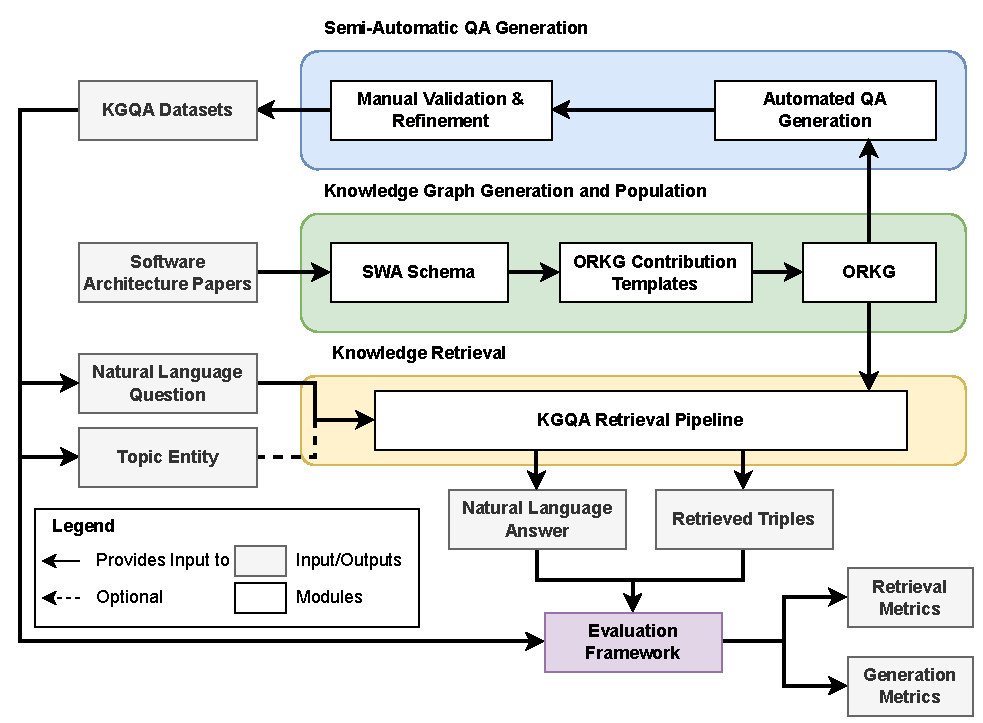
\includegraphics[width=0.95\textwidth]{figures/experiments/orkg/figures-imp_concept_exp.drawio.pdf}
    \caption[Evaluation Concept for Evaluating HubLink on the ORKG]{The overall evaluation concept that we used to perform the experiments on the \gls{orkg} using the proposed HubLink approach and the implemented \gls{kgqa} baseline approaches.}
    \label{fig:implementation_concept}
\end{figure}

This section details the evaluation concept, which we used to perform the evaluation with the objective of assessing the performance of our proposed HubLink approach. The primary objective of this concept is to systematically compare the capabilities of the HubLink retriever against established baseline methods. As indicated in Section~\ref{sec:implementation_orkg}, the \gls{orkg} serves as the underlying \gls{rkg} for these experiments. Furthermore, the \gls{karagen} method \cite{kaplan_combining_2024}, designed for implementing an \gls{llm}-based \gls{qa} system on the \gls{orkg}, forms the basis of the experimental setup. This framework is particularly suitable, as it encompasses the necessary components for applying a \gls{kgqa} retriever to the \gls{orkg}, including data population and retrieval processes. \autoref{fig:implementation_concept} provides a visual overview of the complete experimental design, which we detail in the following.

The general experimental concept starts with the \emph{Knowledge Graph Generation and Population} module. This module is proposed by the \gls{karagen} method and includes the preparation of contribution templates to populate the \gls{orkg} with data. We prepared four such templates, which are described in Section~\ref{sec:contribution_templates}. We fill these templates with data using the \gls{swa} schema detailed in Section~\ref{sec:implementation_orkg}. These populated templates are used by the \gls{sqa} system to automatically fill in the publication data in the \gls{orkg}.

The next module in the evaluation concept is \emph{Knowledge Retrieval}, which also aligns with the principles described in the \gls{karagen} method. In our implementation, the \gls{sqa} system is employed to construct the \gls{kgqa} retrieval pipeline. This enables systematic experimentation by providing a dynamic configuration setup where parameters and pipeline steps can be easily exchanged. The pipeline accepts a natural language question as input and, optionally, a topic entity serving as an entry point into the \gls{orkg}. It then performs knowledge retrieval utilizing either the HubLink retriever or one of five baseline \gls{kgqa} approaches from the literature, detailed in Section~\ref{sec:implementation_baselines}. The parameters that are used for these approaches are chosen by the \emph{Parameter Selection Process}, which is documented in \autoref{ch:parameter_selection_process}. The outputs of the \emph{Knowledge Retrieval} module are a natural language answer and the list of triples retrieved from the graph. These two types of outputs allow the evaluation of both the generation and the retrieval parts of the \gls{kgqa} approach.

The inputs to this system (question and topic entity) are automatically provided to the \gls{kgqa} approach by the \gls{kgqa} dataset. This dataset is the output of the \emph{Semi-Automatic QA Generation} module. Here, the \gls{qa} generation processes implemented in the \gls{sqa} system are used for the generation of \gls{kgqa} pairs (see Section~\ref{sec:implementation_qa_dataset_generation}). During generation, questions are generated in a controlled manner with \gls{llm} assistance using the \gls{orkg} subgraph as the data source. Furthermore, ground-truth data is generated, which is required for the subsequent evaluation phase.

Following the execution of the retrieval pipeline, the output is evaluated within the \emph{Evaluation Framework} module. This final module employs the generated ground-truth data to compute relevant performance metrics. Analysis of these metrics facilitates drawing conclusions regarding the effectiveness and performance characteristics of the evaluated \gls{kgqa} approaches.

\section{Software and Hardware Environment}
\label{sec:exp_prelim_environment}

In this section, we detail the environment in which the experiments for this thesis were executed.

The experiments were performed on the \gls{orkg} in the sandbox environment as detailed in Section ~\ref{sec:implementation_orkg}. However, this does not affect the generality of the results, as the \gls{orkg} serves as a representative example of an \gls{rkg} \cite{verma_scholarly_2023}. Consequently, the broader relevance of the obtained results are not compromised.

Moreover, all experiments were executed within the \gls{sqa} framework, which was developed by the author of the thesis and is detailed in Section~\ref{sec:implementation_sqa_framework}. Both the proposed HubLink retriever and the baseline retrievers were integrated into this framework. To ensure reproducibility, each experiment configuration is specified in a dedicated file using the JSON format. This facilitates straightforward replication of the experimental setup.

With respect to hardware, all experiments were performed in the same consistent hardware and software environment. The system operates on the Linux kernel version \emph{6.1.0-23-amd64}, equipped with a \emph{Intel(R) Xeon(R) Gold 6258R CPU @ 2.70GHz} processor and a \emph{Tesla V100S-PCIE-32GB} graphics processing unit. The implementation relies on a \emph{Python 3.12} environment, with a comprehensive list of software packages and their versions provided in the accompanying replication package \cite{schneider_replication_2025}.

Furthermore, the experimental setup uses both local and remote \glspl{llm}. Local LLMs are managed and executed via the Ollama framework\footnote{\url{https://ollama.com/} [last accessed on 24.02.2025]}. Remote access \glspl{llm} is facilitated through the OpenAI API\footnote{\url{https://platform.openai.com/docs/overview} [last accessed on 24.02.2025]}.


\section{Creating the KGQA Datasets}
\label{sec:implementation_qa_dataset_generation}

To be able to evaluate the retrieval capabilities on diverse retrieval operations and specific use cases in scholarly literature searches, we created new \gls{kgqa} datasets (\hyperref[enum:c3]{\textbf{C3}}). These datasets have been created with the help of the \gls{kgqa} retrieval taxonomy (\hyperref[enum:c3]{\textbf{C3}}) and six use cases using the semi-automatic generation procedures provided by the \gls{sqa} system (see Section~\ref{sec:qa_generator}).

In the following, we first introduce the use cases for scholarly literature search. Then, we explain the different levels of content granularity to clarify the level at which the new datasets are situated. Finally, we introduce the new \gls{kgqa} datasets for four different graph variants.

\subsection{Use Cases for Scholarly Literature Search}
\label{sec:qa_use_cases}

To create the \gls{kgqa} datasets, we prepared use cases. These use cases serve to support the creation process by incorporating real-world scenarios. To guide the development of use cases, we use the categories \emph{Answer Type} and \emph{Condition Type} from the \gls{kgqa} retrieval taxonomy introduced in \autoref{ch:question_catalog}. Here, \emph{Condition Type} refers to the types of conditions provided with a question. The \emph{Answer Type}, on the other hand, implicitly classifies the types of information expected in the answer.

For the design of the use cases, we decided to adapt these two categories to make them better suited to our experimental data. This decision was based on the fact that both categories originally included a large number of classes, which would result in an unmanageable number of use cases if all combinations were considered. Consequently, because the labeled data that we use consists of two types of data (metadata and content data), as shown in \autoref{tab:swa_data_schema}, we apply this distinction by adapting the answer and condition types for the creation of use cases. The result is the following adaptation of the two categories:

\begin{enumerate}[label={}, leftmargin=2.5em]
    \item \textbf{Adapted Answer Type} Classifies whether a question expects a \emph{metadata} or \emph{content data} type in the answer.
    \item \textbf{Adapted Condition Type} Classifies whether a question contains a condition of the \emph{metadata} or \emph{content data} type.
\end{enumerate}

Based on these adapted categories, we present six different use cases tailored to the scholarly literature search task.

\begin{tcolorbox}[title=Use Case 1] % Input:Metadata, Output: Metadata
The first use case reflects the current state of practice in scientific literature search. The researcher seeks additional details about the \emph{metadata} of one or more papers. To find this information, the researcher provides the \gls{kgqa} system with specific metadata information related to the papers they are interested in. In response, the \gls{kgqa} system returns information on other \emph{metadata} attributes of the papers rather than content information.
\end{tcolorbox}

The first use case is classified as \emph{Adapted Condition Type: Metadata} because all questions related to this use case require the answer to meet a specific metadata condition. Furthermore, this use case is categorized as \emph{Adapted Answer Type: Metadata}, as only metadata information is expected in the response.

A practical example of this use case would be a researcher asking for the publications of a specific author. In this case, the name of the author serves as the input constraint, while the returned publication titles represent the output type. Both the input and output consist solely of metadata. Similarly, another example would be a question that provides keywords. The \gls{kgqa} system then has to return the titles of the papers that are related to those keywords. 

Consequently, this use case reflects the current way of searching for scientific artifacts, since state-of-practice search engines like Google Scholar are expected to receive keywords and return titles of publications.

\begin{tcolorbox}[title=Use Case 2] % Input:Metadata, Output: Content
In the second use case, the researcher seeks information about the \emph{content} of one or more papers. In this use case, the researcher provides the \gls{kgqa} system with \emph{metadata} information about the papers and asks a question about their contents. The \gls{kgqa} system is then expected to extract content information related to specific papers that conform to the metadata constraints provided.
\end{tcolorbox}

The second use case is classified as \emph{Adapted Condition Type: Metadata}. However, its category regarding the second dimension is \emph{Adapted Answer Type: Content}, as the answer is expected to contain content information. From a retrieval perspective, we expect this use case to be more challenging, as it requires the \gls{kgqa} system to search through the extensive content information provided in the papers to find the expected answer.

A practical example of this use case would be a researcher asking for the conclusions that a specific publication has drawn. In this case, the name of the publication serves as the input constraint, where the \gls{kgqa} system is required to search the content of the specific publication. The expected output would be the conclusions drawn in the publication, which is content-based information as it requires the \gls{kgqa} system to reason over the content of the publication. Another scenario that would fit this use case would be a researcher asking the \gls{kgqa} system what research problems an author has worked on. In this case, it would require retrieving information from all publications of the author, extracting and aggregating the research problems that each publication investigated, and returning the aggregated list of research problems as the answer.

This use case shows the potential for \gls{kgqa} to help vastly improve the literature search process. By directly allowing researchers to find information based on the contents of a paper, the time and cognitive investment required to manually read through the text of the paper is reduced.

\begin{tcolorbox}[title=Use Case 3] % Input:Content, Output: Metadata
In the third use case, the researcher seeks information about \emph{metadata} of one or more papers. In this use case, the researcher provides the \gls{kgqa} system with \emph{content} constraints about the papers and asks a question about the metadata of the paper. The \gls{kgqa} system is then expected to extract metadata information related to the specific papers mentioned in the question.
\end{tcolorbox}

As opposed to the first two use cases, the third use case is classified as \emph{Adapted Condition Type: Content}. This is because the input constraint is based on content information. However, the expected answer is classified as \emph{Adapted Answer Type: Metadata}, as the answer is expected to only contain metadata information.

A practical example of this use case would be a researcher asking for publications that contain a specific evaluation method or treat the same research problem. Such a question would require inferring over the contents of publications to find out whether they have applied the provided evaluation method or whether they treat the same research problem. In this case, the expected output would be the titles of the publications, which is metadata information, whereas the input constraint is based on the type of expected answer.

This use case demonstrates the potential for improving the current document-centric literature search workflow. This is because a major difficulty faced by researchers is the identification of relevant publications that contain specific information. In the current workflow, researchers have to rely on metadata during their search. However, the desired information is often not explicitly stated in the title or abstract of the publication. Therefore, it is difficult to find the relevant publications using traditional search engines. Consequently, a \gls{kgqa} system that is able to find publications that contain specific content information would be a great improvement for the current literature research workflow.

\begin{tcolorbox}[title=Use Case 4]
In the fourth use case, the researcher seeks information about the \emph{content} of one or more papers. In this use case, the researcher provides the \gls{kgqa} system with content information about the paper, and asks a question about the \emph{content} of the paper. The \gls{kgqa} system is then expected to extract content information related to the specific papers mentioned in the question.
\end{tcolorbox}

The fourth use case has both the \emph{Adapted Condition Type} and \emph{Adapted Answer Type} classified as \emph{Content}. This is because both the input constraints and expected output types are based on content information. 

A practical example of this use case would be a researcher asking for common reference architectures that are proposed when tackling a specific research problem. In this case, the input constraint would be the research problem, while the expected output would be the reference architectures that are proposed in the literature. Both the input and output are content information, as they require reasoning over the content of the publications to find out which reference architectures are proposed for a specific research problem.

This use case is of particular interest when searching for definitions or explanations of specific concepts. In such cases, the location of the information in question is often uncertain, prompting the need to identify both the description and its source for the purpose of referencing it in another academic thesis.

\begin{tcolorbox}[title=Use Case 5]
In the fifth use case, a researcher seeks information about the \emph{content} of one or more papers. In this use case, the researcher provides the retriever with both \emph{metadata and content} information about the papers and asks a question about the content of the paper. The retriever is then expected to extract content information related to the specific papers mentioned in the question.
\end{tcolorbox}

The use cases until now only had a single type of input constraint. However, in the fifth use case, the input constraint is a combination of both \emph{metadata and content} information. This makes the task more difficult for the \gls{kgqa} system. It is now required to search for two different constraint types that might even be stored in different locations in the underlying \gls{kg}. The expected output is \emph{Adapted Answer Type: Content} as the answer is expected to contain content information. 

Practical examples include combinations of the second and fourth use cases. For example, a researcher could ask for a summary of conclusions that publications have drawn in a specific time frame for a specific research problem. In this case, the input constraint would be the research problem and the time frame, which are content and metadata information, respectively. The expected output would be the summary of conclusions that are drawn in the publications, which is content information. 

This use case is particularly interesting in scenarios where a researcher wants to save time by not reading the full text of a publication. Instead of reading the text, the researcher can pose questions to the document in order to retrieve the necessary information.

\begin{tcolorbox}[title=Use Case 6]
In the sixth use case, the researcher seeks information about \emph{metadata} of one or more papers. In this specific use case, the researcher provides the retriever with both \emph{metadata and content} information about the papers, such as the name of an evaluation method and the year of publication, and asks a question about the metadata of the papers. The retriever is then expected to extract metadata information related to the specific papers mentioned in the question.
\end{tcolorbox}

The sixth use case has the same \emph{Adapted Condition Types} as the fifth use case, but the second dimension is \emph{Adapted Answer Type: Metadata} as the answer is expected to contain metadata information. 

The practical examples of this use case are a mixed version of the first and third use cases. For example, a researcher could request publications that have applied a specific evaluation method in a specific research field. In this case, the input constraint would be the evaluation method and the research field, which are content and metadata information, respectively. The expected output would be the titles of publications that have applied the evaluation method in the research field, which is metadata information.

\textit{Note that, as evident from the aforementioned use cases, the Answer Type dimension is not being mixed. According to the \gls{kgqa} retrieval taxonomy, such a question would be designated as a Multiple Intentions question. Splitting this question into two distinct questions is a viable approach to enhance clarity and manage complexity. However, in the interest of maintaining manageable complexity, the multiple intentions are not being considered in the use cases.}

\subsection{Overview of Content Granularity}
\label{sec:content_granularity}

When creating datasets, it is useful to classify the level of granularity the data contains. This helps to provide a better understanding of the content of the dataset. For this purpose, we introduce four levels of granularity, which differ in their degree of abstraction:

\begin{enumerate} 
    \item \textbf{Document-based:} The current standard for distributing literature online. Publications are stored as PDF files in a database together with their metadata. Users locate publications using the metadata and then extract relevant information from the documents themselves by reading the provided texts. 
    \item \textbf{Chunk-based:} Originating from \gls{rag} \cite{lewis_retrieval-augmented_2021}, this approach divides documents into smaller chunks and embeds them into a vector space. Relevant chunks are retrieved from the database using nearest-neighbor search queries.
    \item \textbf{Statement-based:} Here, concise summaries or statements are extracted from publications and stored directly in a database. 
    \item \textbf{Label-based:} The highest level of abstraction, where publications are classified using labels, which may include hierarchical structures. These labels give readers a quick overview of the content of a publication. 
\end{enumerate}

Using this classification, we assign the datasets that we used for our experiments to the \emph{Label-based} abstraction level. This is because they consist of extracted terms structured according to a predefined schema as defined in \autoref{tab:swa_data_schema}.

\subsection{Dataset Creation Process}
\label{sec:label_based_qa_dataset}

Contribution \textbf{C2} of this thesis are \gls{kgqa} datasets, which we used to carry out the experiments. These \gls{kgqa} datasets were created using the data from the publication dataset introduced in Section~\ref{sec:experiments_dataset}. For their creation, the data was first loaded into the \gls{orkg}, and then \gls{kgqa} pairs were generated using the semi-automated \gls{kgqa} generation strategy described in Section~\ref{sec:qa_generator}. In the following, we present the creation process and the key characteristics of these datasets.

\subsubsection{Dataset Structure} 

The datasets consist of \gls{kgqa} pairs. Each pair includes the question itself together with the corresponding \emph{ground-truth} data. This data is used during the evaluation to determine whether the answer and the data retrieved by the \gls{kgqa} approach are correct. In this context, the ground truth represents one possible valid answer to the question, as well as a collection of triples needed to answer it. In addition to the question and the ground truth, each \gls{kgqa} pair also includes further metadata. This encompasses a \emph{topic entity} that can serve as an entry point into the graph for the retriever, the \glspl{doi} of the papers referenced in the question, and the template used to generate the question. The pairs are also classified according to use case, semi-typed nature, and the categories defined in the taxonomy.

\subsubsection{Question Diversity}

To ensure that the questions in the \gls{kgqa} datasets exhibit a high degree of variability that allows meaningful conclusions about the capabilities of a \gls{kgqa} system, we structured the datasets considering multiple dimensions. First, we use the \emph{use cases} described in Section~\ref{sec:qa_use_cases} to map each question to a realistic application scenario. During the creation phase, we assigned questions to each of the six use cases to ensure a balanced distribution between them. To further reflect the retrieval capabilities required for each question, we incorporated the \emph{Retrieval Operation} category from the \gls{kgqa} retrieval taxonomy introduced in \autoref{ch:question_catalog}. Each question is assigned to a specific retrieval operation, ensuring that operations are covered evenly. 

Additionally, the dataset distinguishes between \emph{untyped} and \emph{semi-typed} questions. This distinction is meant to assess how well a retriever can handle synonyms or missing type information:

\begin{itemize}
    \item \textbf{Semi-Typed Questions} Each question in the dataset targets specific triples in the \gls{kg}, with each triple consisting of a subject, predicate, and object. Depending on the triple, either the subject or the predicate may carry type information about the object. For example, the requested triple $(Research Object Entity, Name, Reference Architecture)$, requires the question to specify that the reference architecture is a research object.
    
    \item \textbf{Untyped Questions} In contrast, \emph{untyped} questions do not include the type information. Using the same example, the question would simply ask about the reference architecture without stating that it is a research object. This increases the difficulty of retrieval because the retriever must infer the object type based solely on the object name.
\end{itemize}


\subsubsection{Restrictions} 

To keep the datasets manageable in terms of complexity, certain constraints were applied during the creation. First, the number of golden triples needed to answer a question was limited to a maximum of 10. This limitation ensures that questions do not require information spread across the entire dataset. Without this restriction, answering broad questions would require extensive aggregation, resulting in runtimes that are too long for the scope of a master thesis.

Furthermore, it is essential that the retriever parameters are set in such a way that the retrievers can fully answer the given questions. By limiting the number of golden triples, we can ensure that this is the case. Consequently, the chosen threshold of 10 represents a compromise between the efficiency of the retrievers and the expressiveness of the questions. A higher threshold would require increasing retriever parameters, such as maximum depth or width, leading to longer runtimes. A lower threshold, on the other hand, would reduce the informativeness of the questions or even make some of them unanswerable. Therefore, selecting a limit of ten triples strikes a balance between maintaining acceptable runtimes and preserving the relevance and feasibility of the questions.

\begin{table}[t]
\centering
\begin{tabular}{lccccccc}
\toprule
\textbf{} & \multicolumn{6}{c}{\textbf{Use Cases}} \\
\cmidrule(lr){2-7}
\textbf{Retrieval Operation} & \textbf{1} & \textbf{2} & \textbf{3} & \textbf{4} & \textbf{5} & \textbf{6} \\
\midrule
aggregation   & 4 & 4 & 4 & 4 & 4 & 4 \\
basic         & 4 & 4 & 4 & 1 & 4 & 1 \\
comparative   & 4 & 4 & 4 & 4 & 4 & 4 \\
counting      & 4 & 4 & 4 & 4 & 4 & 4 \\
negation      & 0 & 0 & 4 & 4 & 4 & 4 \\
ranking       & 4 & 4 & 4 & 4 & 4 & 4 \\
relationship  & 4 & 4 & 4 & 4 & 4 & 4 \\
superlative   & 0 & 0 & 4 & 4 & 4 & 4 \\
\bottomrule
\end{tabular}
\caption[Distribution of Question Templates]{Distribution of question templates across the use case and retrieval operation dimensions.}
\label{tab:distribution_of_question_templates}
\end{table}

\subsubsection{Template Questions} 

To utilize the semi-automatic \gls{kgqa} generation described in Section~\ref{sec:qa_generator}, template questions are required. For the datasets, a total of 170 different template questions were created manually, the full list of which is available in our replication package (see \cite{schneider_replication_2025}). As mentioned previously, these questions were diversified along the dimensions of the use case and retrieval operation. The precise distribution of these template questions is shown in \autoref{tab:distribution_of_question_templates}. For most combinations of use case and retrieval operation, four template questions were generated, although there are some exceptions. Specifically, for the use cases four and six, only two suitable examples were found for the \emph{Basic} operation. Additionally, for use cases one and two, no suitable template questions were identified for the \emph{Negation} and \emph{Superlative} classes that were meaningful and below the threshold of ten golden triples.

Regarding the semi-typed nature of the questions, the dataset contains 86 semi-typed and 84 untyped questions. Generally, an equal number of semi-typed and untyped questions were created for each combination of use case and retrieval operation, with the exception of the individual questions for use cases four and six as mentioned above.

\subsubsection{Classification According to KGQA Retrieval Taxonomy} 

According to the classification following the \gls{kgqa} retrieval taxonomy described in \autoref{ch:question_catalog}, the distribution is as follows: Within the \emph{Condition Type} category, 133 questions were classified as \emph{Named Entity} and 37 as \emph{Named Entity, Temporal}. This indicates that two types of constraints must be considered by the retriever: either solely the consideration of a named entity or additionally a temporal constraint.

For the \emph{Answer Format} category, the dataset comprises 61 \emph{Enumerative}, 58 \emph{Simple}, and 51 \emph{Explanatory} questions. The classification according to \emph{Graph Representation} shows that 152 questions belong to the \emph{Multi-Fact} type, meaning they require multiple triples for their answer, while 18 questions are categorized as \emph{Single-Fact}, requiring only one triple.

In the \emph{Answer Type} category, 86 questions expect an answer of type \emph{Named Entity}, 20 questions require a \emph{Quantitative} answer, two questions anticipate a \emph{Boolean} answer, and two additional questions have an \emph{Other Type} of response. Furthermore, the dataset includes questions with more complex answer types: 24 questions expect either \emph{Description} combined with \emph{Quantitative} (\emph{Description, Quantitative}) or \emph{Description} with \emph{Named Entity} (\emph{Description, Named Entity}). Additionally, 13 questions require answers of the type \emph{Description, Quantitative, Temporal}, and 8 questions expect answers of the type \emph{Description, Named Entity, Temporal}, which means that they also require a year.

With respect to the \emph{Intention Count} category, the dataset exclusively contains \emph{Single Intention} questions, as multiple intentions were not considered. For the \emph{Question Goal} category, due to insufficient variability in the publication data, only the class \emph{Information Lookup} applies. Regarding \emph{Answer Credibility}, all the questions meet the \emph{Objective} criterion.

\subsubsection{Dataset Creation} 
To generate the datasets, we used the semi-automatic cluster and subgraph-based generation methods introduced in Section~\ref{sec:qa_generator}. Based on the template question and the provided generation methods, we generated a total of 170 initial questions for the graph variant \hyperref[enum:gv2]{\textbf{GV2}}. Then, each question and the corresponding ground truth were reviewed manually to ensure that both the question and the generated golden answers are consistent and grammatically correct. To further ensure quality, an additional \gls{llm}-based feedback script was employed, which checked each question and answer to provide feedback for changes if necessary.

After the quality of each question-answer pair was verified, we manually classified each question with the remaining categories of the \gls{kgqa} retrieval taxonomy. Then, we employed the \emph{conversion} scripts introduced in Section~\ref{sec:orkg_ensuring_repeatability} to generate the \gls{kgqa} datasets for the graph variants \hyperref[enum:gv1]{\textbf{GV1}}, \hyperref[enum:gv3]{\textbf{GV3}}, and \hyperref[enum:gv4]{\textbf{GV4}}.




\section{Evaluation Framework and Metrics}
\label{sec:exp_prelim_evaluation_framework}

The \gls{kgqa} approaches that we are testing in our thesis conform to the principles of \gls{rag}, because they retrieve information that is then used to improve the generation of an answer. Consequently, we employ an evaluation framework for \gls{rag}-based systems. A popular framework is \gls{rgar} \cite{yu_evaluation_2024}, which will serve as the basis for structuring our evaluation. The framework is divided into three modules. The first module, called \emph{Evaluation Target}, defines the direction of the evaluation. The second module is \emph{Evaluation Dataset}, which outlines how the datasets were created and selected. The last module is \emph{Evaluation Metric}, which presents the specific metrics used to evaluate the targets based on the datasets. 

In the following, we first introduce the evaluation targets differentiating between retrieval and generation objectives. Then, we briefly explain the datasets that were applied in the experiments. Finally, we introduce the \gls{gqm} plan that shows how each target is evaluated using specific questions and metrics.


\subsection{Evaluation Targets}
\label{sec:evaluation_targets}

This section introduces the evaluation targets, which are the constructs intended to be evaluated during the evaluation. Each evaluation target is defined using \glspl{eo} and \glspl{gt}.

\subsubsection{Outputs and Ground Truth}

\glspl{eo} are the actual outputs of the \gls{kgqa} approach, while \glspl{gt} are the expected outputs as defined in the \gls{kgqa} dataset. We define the following \glspl{eo} and \glspl{gt} for our evaluation:

\begin{enumerate}[label={}, leftmargin=5em]
    \item[\textbf{EO1}] \label{enum:eo1} Retrieved Triples
    \item[\textbf{EO2}] \label{enum:eo2} Generated Answer
    \item[\textbf{GT1}] \label{enum:gt1} Golden Triples
    \item[\textbf{GT2}] \label{enum:gt2} Golden Answer
\end{enumerate}

Each \gls{kgqa} approach returns two types of outputs in our setting. The first output is \textbf{EO1}, which represents the triples that have been retrieved from the \gls{orkg} and rated by the approach as relevant to answering the provided question. Second, \textbf{EO2} is the answer that has been generated by an \gls{llm} based on the retrieved triples and the question.

To evaluate the outputs of the retriever, the \gls{kgqa} dataset provides two types of ground truth data. First, \textbf{GT1} are the golden triples, which are exactly those triples that are required to fully answer the question that was asked. Consequently, the retriever has to find all golden triples to be entirely successful at the retrieval task. Second, \textbf{GT2} is a golden answer formulated in natural language, which provides a response to the question and is based on the golden triples. 

\subsubsection{Evaluation Targets}
The combination of \glspl{eo} and \glspl{gt} generates the evaluation targets, which are subdivided into targets for retrieval (\emph{ReT}) and for generation (\emph{GeT}):

\begin{enumerate}[label={}]
    % Triples to Golden Triples
    \item \textbf{ReT1}\label{enum:ret1} EO1 \(\leftrightarrow \) GT1
     % Gen Answer to Golden Answer
    \item \textbf{GeT1}\label{enum:get3} EO2 \(\leftrightarrow \) GT2
    % Gen Answer to Question
    \item \textbf{GeT2} \label{enum:get1} EO2 \(\leftrightarrow \) Question
    % Gen Answer to Triples
    \item \textbf{GeT3} \label{enum:get2} EO2 \(\leftrightarrow \) GT1
\end{enumerate}

The targets introduced above guide the evaluation process. The retrieval target (\hyperref[enum:get1]{\textbf{ReT1}}) assesses the effectiveness of the context retrieval phase by comparing the retrieved triples (\hyperref[enum:eo1]{\textbf{EO1}}) with the golden triples (\hyperref[enum:gt1]{\textbf{GT1}}). This evaluation focuses on accuracy, relevance, and robustness. Here, accuracy is about the extent to which the retrieval approach is capable of fetching the desired triples (\hyperref[enum:get1]{\textbf{GT1}}) from the graph. Relevance refers to the degree to which the retrieved triples (\hyperref[enum:get1]{\textbf{EO1}}) correspond to the golden triples (\hyperref[enum:get1]{\textbf{GT1}}), where more irrelevant triples result in lower overall relevance. Finally, robustness refers to the ability of the retrieval system to maintain consistent performance in terms of accuracy and relevance despite variations encountered in the complexity of input questions (e.g., phrasing, the presence or absence of explicit type information, diverse use case requirements, and structural or lexical variability) across different knowledge graph schemas. The general intent behind \hyperref[enum:get1]{\textbf{ReT1}} is therefore to quantify how well the retriever identifies the correct information and how resilient its performance is under various operational conditions.

With regard to the generation targets, \hyperref[enum:get1]{\textbf{GeT1}} evaluates the quality of the generated answer by assessing its semantic and factual alignment with the reference ground truth answer (\hyperref[enum:get1]{\textbf{GT2}}). This target aims to measure how closely the generated answer of the system (\hyperref[enum:get1]{\textbf{EO2}}) matches an ideal and correct answer derived from the ground truth. The focus is on both the meaning and the accuracy of the information presented. High performance on this target indicates that the system can produce answers that are similar to a known correct answer.

\hyperref[enum:get2]{\textbf{GeT2}} evaluates how well the generated answer (\hyperref[enum:get1]{\textbf{EO2}}) aligns with the intent and content requirements of the input question. This involves assessing whether the answer directly addresses the topic posed by the question and fulfills any specific instructions or constraints given, such as performing a ranking or counting operation. Consequently, this target measures the usefulness and appropriateness of the generated answer in the context of the question.

Finally, \hyperref[enum:get3]{\textbf{GeT3}} evaluates the faithfulness and adherence to the source material of the generated answer (\hyperref[enum:get1]{\textbf{EO2}}) relative to the retrieved triples (\hyperref[enum:get1]{\textbf{EO1}}). It evaluates whether the statements and claims made in the generated answer accurately and exclusively reflect the information present within the retrieved triples. 

\subsection{Evaluation Datasets}
\label{sec:evaluation_datasets}

To evaluate the defined targets, datasets are needed to conduct the experiments. In Section~\ref{sec:implementation_qa_dataset_generation} we document the creation of \gls{kgqa} datasets. These datasets have been used to conduct the experiments and evaluate the targets.

\subsection{Evaluation Plan}
\label{sec:evaluation_goals_and_metrics}

This section details the evaluation plan designed to assess the performance of the proposed HubLink system against baseline approaches. Following the introduction of the evaluation targets in Section~\ref{sec:evaluation_targets}, we adopt the \gls{gqm} method \cite{basili_methodology_1984,basili_software_1992}. Consequently, we present a detailed \gls{gqm} plan that systematically links each evaluation target (serving as a goal) with specific questions, which are in turn addressed using a defined set of quantitative metrics. To aggregate the metrics across all questions, we are using the \emph{macro-averaging} strategy (see Section~\ref{sec:fundamentals_evaluation_rag}) because it attributes equal weight to each individual question without favoring those questions that request more triples.

In the following, we present each of the goals with their corresponding set of questions and metrics. We begin with the retrieval, followed by the generation.



\subsubsection{Evaluation of the Retrieval Performance} 

The initial evaluation target, \hyperref[enum:ret1]{\textbf{ReT1}}, centers on assessing the relevance and robustness of the contexts retrieved by HubLink. Several questions arise from this goal, evaluated using a suite of seven metrics. Standard information retrieval metrics, namely \emph{Precision}, \emph{Recall}, and \emph{F1} are calculated based on the formulas presented by \textcite{yu_evaluation_2024}. The determination of \gls{tp}, \gls{fp}, and \gls{fn} involves comparing the triples retrieved by the system with the ground-truth triples provided within the reference \gls{kgqa} dataset. The \emph{Accuracy} metric is omitted from this evaluation, as its calculation requires knowledge of \gls{tn}, which requires a complete listing of all irrelevant contexts, which is not available in our \gls{kgqa} datasets.

To evaluate the ability of the retriever to rank relevant contexts highly, rank-aware metrics are incorporated. Specifically, \emph{MAP@k} and \emph{MRR@k} are adapted from the implementations of \textcite{tang_multihop-rag_2024}. The \emph{Hits@k} metric is implemented following the definition provided by the AmpliGraph library\footnote{\url{https://docs.ampligraph.org/en/1.2.0/generated/ampligraph.evaluation.hits_at_n_score.html} [last accessed on 17.01.2025]}. In addition, \emph{EM@k} is included, calculated according to the definition of \textcite{ibrahim_survey_2024}. 

With regard to the required parameter $k$ that determines the number of top contexts considered, we have set this parameter to 10. This choice reflects the maximum number of ground truth triples associated with any single question in our \gls{kgqa} datasets, as detailed in Section~\ref{sec:label_based_qa_dataset}.

Furthermore, we test the environmental impact of the retrieval using the absolute, relative, and delta carbon emissions using the metrics specified by \cite{kaplan_responsible_2025}. The tracking of the emissions is facilitated by the Codecarbon library\footnote{\url{https://github.com/mlco2/codecarbon} [Accessed: 2025-01-17]}, which tracks the \emph{CPU Energy Consumption}, \emph{GPU Energy Consumption}, and \emph{RAM Energy Consumption}, measured in watts and then converts those measurements to estimate the total \emph{Carbon Emissions} as \(CO_2\) equivalent. Moreover, to evaluate runtime and token costs, we measure \emph{System Latency} as the total time taken to retrieve the context and generate an answer while also tracking the number of \emph{LLM Tokens} consumed during the retrieval and generation phases.


% Beyond the \gls{gqm} framework, several measurements are tracked to quantify practical operational aspects. \emph{System Latency} is measured as the total time elapsed to retrieve the context and generate an answer. Sustainability considerations are addressed by tracking energy consumption, specifically \emph{CPU Energy Consumption}, \emph{GPU Energy Consumption}, and \emph{RAM Energy Consumption}, measured in watts. These energy measurements are aggregated to estimate the total \emph{Carbon Emissions} as \(CO_2\) equivalent. The tracking of energy and emissions is implemented using the Codecarbon library\footnote{\url{https://github.com/mlco2/codecarbon} [Accessed: 2025-01-17]}. Finally, the computational cost associated with the usage of the \gls{llm} is monitored by tracking the number of \emph{LLM Tokens} consumed during the retrieval and generation phases.


\subsubsection{Evaluation of the Generation Performance}

Transitioning to answer generation, the target \hyperref[enum:get1]{\textbf{GeT1}} focuses on comparing the factual and semantic similarity between the generated answer of the \gls{kgqa} approach and the golden answer in the \gls{kgqa} dataset. Lexical similarity is measured using \emph{BLEU}\footnote{\url{https://pypi.org/project/sacrebleu/} [last accessed on 17.01.2025]} and \emph{ROUGE}\footnote{\url{https://pypi.org/project/rouge-score/} [last accessed on 17.01.2025]}, employing their respective standard Python implementations. Semantic similarity is assessed using \emph{BertScore}\footnote{\url{https://github.com/Tiiiger/bert_score} [last accessed on 17.01.2025]} utilizing the official implementation that provides Precision, Recall, and F1 variants based on contextual embeddings. Further evaluation leverages \gls{llm}-as-a-judge metrics provided by the RAGAS framework\footnote{\url{https://github.com/explodinggradients/ragas} [last accessed on 17.01.2025]}. This includes \emph{Factual Correctness}, where an \gls{llm} decomposes both the generated and reference answers into claims to calculate Precision, Recall, and F1 based on the comparisons of those claims \cite{es_ragas_2023}. We further use the \emph{Semantic Similarity} metric, which calculates the cosine similarity and the \emph{String Similarity} metric, which calculates the Levenshtein distance between the generated answer and the golden answer. Both metrics are also provided by the RAGAS framework.

The subsequent generation target, \hyperref[enum:get2]{\textbf{GeT2}}, addresses the alignment of the generated answers with the intent of the question, encompassing both semantic content and instructional constraints. This target involves two specific questions. The first, referring to semantic alignment, is evaluated using the \emph{Answer Relevancy} metric from RAGAS. This metric uses an \gls{llm} to generate plausible questions based solely on the generated answer and then measures the semantic similarity (cosine similarity) between these generated questions and the original question \cite{es_ragas_2023}. The rationale is that a relevant answer should allow an accurate reconstruction of the original query. The second question, which focuses on adherence to instructional intent (e.g., performing a ranking task as requested), is assessed using a custom implementation that we developed on our own. In this process, an \gls{llm} evaluates the generated answer against the specific instructions embedded within the question to determine the degree of compliance.

The final generation target \hyperref[enum:get3]{\textbf{GeT3}} concerns the faithfulness of the generated answer to the information contained within the retrieved contexts. This is evaluated using the \emph{Faithfulness} metric from the RAGAS framework. This metric utilizes an \gls{llm} to break down the generated answer into individual statements and verifies each statement against the provided retrieved context  \cite{es_ragas_2023}. This means that the metric evaluates whether the answer was actually derived from the context or from the internal knowledge of the \gls{llm}. We use this to evaluate whether the triples that were retrieved are actually reflected in the generated answer. 

\vspace{\medskipamount}
{\large\textbf{Goal-Question-Metric Plan:}} 
\label{sec:evaluation_gqm_plan}

\textbf{Ret1} Assess the relevance and robustness of retrieved contexts in scholarly literature search.
\begin{enumerate}[label={}]
    \item \textbf{Q1} To what extent does the HubLink retrieval algorithm improve context relevance and accuracy compared to baseline KGQA methods in scholarly literature search?
    \begin{enumerate}[label={}]
        \item \textbf{M1.1} Precision, \textbf{M1.2} Recall, \textbf{M1.3} F1, \textbf{M1.4} Hits@k, \textbf{M1.5} EM@k, \textbf{M1.6} MRR@k, \textbf{M1.7} MAP@k
    \end{enumerate}
    \item \textbf{Q2} How does retrieval performance vary with the complexity of operations required by different scholarly questions?
    \begin{enumerate}[label={}]
        \item \textbf{(see Q1.1)}
    \end{enumerate}
    \item \textbf{Q3} How does retrieval performance vary across distinct scholarly literature-search use cases?
    \begin{enumerate}[label={}]
        \item \textbf{(see Q1.1)}
    \end{enumerate}
    \item \textbf{Q4} What impact does the presence or absence of explicit type information in questions have on the retrieval performance?
    \begin{enumerate}[label={}]
        \item \textbf{(see Q1.1)}
    \end{enumerate}
    \item \textbf{Q5} How robust is the proposed approach to structural and lexical variability across alternative knowledge graph schema representations?
    \begin{enumerate}[label={}]
        \item \textbf{(see Q1.1)}
    \end{enumerate}
    \item \textbf{Q6} How efficient is the proposed approach considering runtime and language model tokens required when compared to baseline KGQA methods?
    \begin{enumerate}
        \item \textbf{M1.8} Runtime per question, \textbf{M1.9} LLM tokens per question
    \end{enumerate}
    \item \textbf{Q7} How does the proposed approach compare with regard to the environmental impact when compared to baseline KGQA methods?
    \begin{enumerate}
        \item \textbf{M1.10} Absolute carbon emissions, \textbf{M1.11} Relative carbon emissions, \textbf{M1.12} Delta carbon emissions
    \end{enumerate}
\end{enumerate}
% 
\textbf{GeT1} Evaluate how well the generated answer aligns semantically and factually with reference answers.
\begin{enumerate}[label={}]
    \item \textbf{Q8} How semantically and factually consistent are the generated answers of the proposed approach when compared to answers generated by baseline KGQA approaches?
    \begin{enumerate}[label={}]
        \item \textbf{M2.1} BLEU, \textbf{M2.2} ROUGE, \textbf{M2.3} Semantic Similarity, \textbf{M2.4} String Similarity, \textbf{M2.5} Bert Precision, \textbf{M2.6} Bert Recall, \textbf{M2.7} Bert F1, \textbf{M2.8} Factual Correctness Precision, \textbf{M2.9} Factual Correctness Recall, \textbf{M2.10} Factual Correctness F1 \\
    \end{enumerate}
\end{enumerate}
%
\textbf{GeT2} Evaluate how well the generated answer aligns with the intent and content of the question.
\begin{enumerate}[label={}]
    \item \textbf{Q9} To what extent do the answers generated by HubLink reflect the semantic intent of scholarly questions when compared to baseline KGQA approaches?
    \begin{enumerate}[label={}]
        \item \textbf{M3.1} Answer Relevancy
    \end{enumerate}
    \item \textbf{Q10} To what extent do the generated answers follow the instructional expectations of scholarly questions when compared to baseline KGQA approaches?
    \begin{enumerate}[label={}]
        \item \textbf{M3.2} Instruction Following
    \end{enumerate}
\end{enumerate}
% 
\textbf{GeT3} Evaluate how well the generated answer aligns with the retrieved context.
\begin{enumerate}[label={}]
    \item \textbf{Q11} To what extent are generated answers of HubLink faithful to the retrieved context and free from unsupported claims when compared to baseline KGQA approaches?
    \begin{enumerate}[label={}]
        \item \textbf{M4.1} Faithfulness
    \end{enumerate}
\end{enumerate}





\section{Dependent and Independent Variables}
\label{sec:exp_prelim_variables}
This section describes the independent and dependent variables of our experiments.

\paragraph{Independent Variables:} These variables encompass the specific experimental configurations that are systematically varied between runs while performing the evaluation. The key independent variables include the choice of the core retrieval algorithm, modifications to its parameters, the specific dataset used for evaluation, the underlying knowledge base, and the selected \gls{llm}. These variables represent the factors that are manipulated to observe their effect on overall performance.

\paragraph{Dependent Variables:} The dependent variables represent those constructs that we are interested in improving. Consequently, these constitute the quantitative performance measures used to assess the outcomes of different experimental configurations and directly correspond to the metrics detailed in the evaluation plan (see Section~\ref{sec:evaluation_goals_and_metrics})

The experimental methodology involves the execution of a series of tests in which specific configurations of independent variables (pipeline components and parameters) are applied. For each configuration, the dependent variables (retrieval, generation, and operational metrics) are measured. The primary objective of this process is to analyze the collected data to determine the influence of variations in the independent variables on the observed system performance in the different categories of dependent variables. Because each \gls{kgqa} approach has a different set of parameters (independent variables), we employ a \emph{Parameter Selection Process} to choose the appropriate values for our subsequent experiments. The selection process is documented in the following \autoref{ch:parameter_selection_process}.



